\chapter{Paralelizaci\'{o}n de la aproximaci\'{o}n del algoritmo \textit{level set}}

Las clases a modificar sobre el trabajo de Ofeli \cite{ofeli} para poder realizar una implementaci\'{o}n paralela son: \textit{ActiveContour}, \textit{ACwithoutEdges} y \textit{list}. De manera que se paralelizar\'{a} el c\'{o}digo para realizar la segmentaci\'{o}n de im\'{a}genes a escala de grises, ya que en un principio el cliente s\'{o}lo est\'{a} interesado en este tipo de im\'{a}genes. A\'{u}n as\'{i}, una vez realizada la segmentaci\'{o}n para este tipo de im\'{a}genes ser\'{i}a muy sencillo poder aplicarlo a im\'{a}genes a color, ya que, como se ha visto en el cap\'{i}tulo anterior, la mayor\'{i}a de las funciones son comunes a la clase \textit{ActiveContour}. 

La segmentaci\'{o}n a resolver es en cierto modo <<poco>> costosa, ya que se realiza en unos cuantos segundos. Las m\'{a}quinas disponibles para la realizaci\'{o}n de este proyecto son una m\'{a}quina propia del cliente  para realizar peque\~{n}as pruebas (4 \textit{cores}), la m\'{a}quina propia del autor de esta memoria (2 \textit{cores}) y una m\'{a}quina de la Facultad de Inform\'{a}tica de la UPV/EHU (48 \textit{cores}). Por todo ello, se ha elegido realizar la paralelizaci\'{o}n mediante  OpenMP\cite{openmp} por lo que las pruebas se realizar\'{a}n en m\'{a}quinas con una arquitectura SMP. Adem\'{a}s, esta elecci\'{o}n puede suponer una ventaja a la hora de querer realizar la segmentaci\'{o}n de las im\'{a}genes de un v\'{i}deo ya que se podr\'{i}a combinar con el est\'{a}ndar MPI como se explicar\'{a} en la secci\'{o}n \ref{propuestaDeMejora}. Para aprovechar las mejores opciones que esta API(\textit{Application Programming Interface}) nos ofrece, es decir, para poder sacarle el m\'{a}ximo rendimiento posible al algoritmo, se ha consultado un tutorial de \textit{Livermore Computing Center} \cite{live1} ya que es una fuente fiable.

\section{Planteamiento de la paralelizaci\'{o}n}

Para empezar, se ha tenido que determinar donde es necesaria la paralelizaci\'{o}n. Fij\'{a}ndonos un poco en el c\'{o}digo de cada ciclo, ya sea el de evoluci\'{o}n del contorno o el del suavizado \textit{Gaussiano}, tiene en total cuatro bucles o recorridos de las listas. Estos recorridos son los que tendremos que paralelizar ya que son los <<cuellos de botella>> de este algoritmo. N\'{o}tese que la cantidad de puntos que contienen las listas puede ser muy grande a medida que se aumenta el tama\~{n}o de la imagen. Adem\'{a}s, se deber\'{a}n de hacer cuatro recorridos \'{u}nicamente para expandir el contorno un p\'{i}xel hacia fuera o hacia dentro. 

Una vez aclarada esta cuesti\'{o}n se debe observar m\'{a}s detalladamente cada recorrido de las listas en busca de condiciones de carrera. As\'{i} pues, se desglosan los cuatro recorridos comunes a los dos ciclos por separado:

\begin{enumerate}
	\item \textbf{Primer bucle}: recorrido de la lista $L_{out}$. La operaci\'{o}n que se lleva a cabo en este bucle es la denominada \textit{switch\_in()} y se realiza/ejecuta solo si se cumple cierta condici\'{o}n dependiente \'{u}nicamente de la velocidad del punto. Como recuerdo, esta operaci\'{o}n trasladaba el punto tratado, perteneciente a la lista $L_{out}$, a la lista $L_{in}$ (al comienzo de la lista) y a\~{n}ad\'{i}a la nueva vecindad de este punto a $L_{out}$ (tambi\'{e}n al comienzo de la lista).
	\begin{enumerate}
		\item Problema:	
			\begin{enumerate}
				\item Cuando dos \textit{threads} quieran cambiar el punto que est\'{a}n tratando de la lista $L_{out}$ a la lista $L_{in}$, al estar trabajando con listas ligadas, el querer a\~{n}adir al mismo tiempo dos puntos al comienzo de la lista dar\'{i}a un problema con los punteros. Por lo tanto, esta operaci\'{o}n de cambiar de lista un punto deber\'{a} de hacer at\'{o}micamente. 
				\item Al haber cambiado un punto de una lista a otra, en nuestro caso de $L_{out}$ a $L_{in}$ se a\~{n}ade la nueva vecindad de ese punto a $L_{out}$. Pasa exactamente lo mismo que en el anterior caso, cuando varios \textit{threads} est\'{a}n a\~{n}adiendo puntos vecinos al principio de la lista habr\'{a} un problema con los punteros. 
				\item Otro problema relacionado con el anterior puede suceder cuando dos puntos de diferentes \textit{threads} quieran a\~{n}adir al mismo vecino al mismo tiempo. Esto puede suceder dependiendo de la morfolog\'{i}a de las islas de la imagen. V\'{e}ase la figura \ref{mismoVecino} donde se supone que los puntos de la parte superior los procesa el primer \textit{thread} y los de la parte inferior el segundo \textit{thread}. En este ejemplo el punto A ser\'{i}a un vecino com\'{u}n para el punto directamente superior a \'{e}l tratado por el primer \textit{thread} y para el punto directamente inferior a \'{e}l, tratado por el segundo \textit{thread}. Si esto ocurriese, podr\'{i}a haber puntos repetidos en la lista, poniendo en riesgo su consistencia. 
			\end{enumerate}
		\item Soluci\'{o}n:
			\begin{enumerate}
				\item La soluci\'{o}n m\'{a}s sencilla para resolver los dos primeros problemas ser\'{i}a poner secciones cr\'{i}ticas a la hora de a\~{n}adir puntos a las listas. Obviamente esto resuelve el problema pero el rendimiento ser\'{i}a pr\'{a}cticamente el de la ejecuci\'{o}n en serie si no es incluso peor que \'{e}ste por el \textit{overhead} que pueda suponer la gesti\'{o}n de la secci\'{o}n cr\'{i}tica. Entonces, si el problema son las operaciones con las listas, est\'{a} claro que cada \textit{thread} tendr\'{a} que tener una estructura propia donde a\~{n}adir esos puntos para poder evitar estos dos primeros problemas. As\'{i} pues, se ha decidido <<partir>> las listas $L_{out}$ y $L_{in}$ en funci\'{o}n del numero de \textit{threads}, para que cada uno trabaje con sus listas. Al final del ciclo habr\'{a} que volver a unir todos los <<trozos>> que tenga cada \textit{thread} para volver a reconstruir las listas. Estas operaciones pueden suponer un sobrecoste alto en cuanto a la versi\'{o}n serie, a\'{u}n as\'{i}, vali\'{e}ndonos de las posibilidades que nos ofrecen las listas enlazadas podemos llegar a hacer estas dos operaciones casi en tiempo constantes. En el caso de no poder hacerlas eficientemente se podr\'{i}an realizar cada cierto n\'{u}mero de ciclos, aunque esto tendr\'{a} como consecuencia que la carga est\'{e} desbalanceada entre distintos \textit{threads}, ya que cada uno puede quitar o a\~{n}adir una diferente cantidad de p\'{i}xeles. Habr\'{a} que buscar un equilibrio para poder hacer un buen \textit{load balancing}. 
				\item En cuanto al tercer problema, no queda m\'{a}s opci\'{o}n que resolverlo mediante una secci\'{o}n cr\'{i}tica, en la que se asegure la inserci\'{o}n \'{u}nica del vecino. 
			\end{enumerate}
	\end{enumerate}
	\item \textbf{Segundo bucle}: limpieza de la lista $L_{in}$. En este recorrido se comprueba si hay alg\'{u}n punto redundante en base a su vecindad y si alguno lo es se quita de la lista. 
	\begin{enumerate}
		\item Problema:
			\begin{enumerate}
				\item Al realizar el borrado de un punto de la lista, y al trabajar con listas enlazadas, puede que otro \textit{thread} este tratando el elemento posterior al que se vaya a eliminar y se tenga problema con los punteros de nuevo. Hay que decir tambi\'{e}n que esta situaci\'{o}n solo se podr\'{a} dar con los puntos <<frontera>>, es decir, con el \'{u}ltimo punto de un \textit{thread} y el primero de otro.
			\end{enumerate}
		\item Soluci\'{o}n: 
			\begin{enumerate}
				\item Este problema quedar\'{i}a resuelto con la soluci\'{o}n propuesta para los primeros problemas del primer bucle, es decir, el troceado de las listas en base al n\'{u}mero de \textit{thread}: un trozo por cada uno de ellos.
			\end{enumerate}
	\end{enumerate}
	\item \textbf{Tercer bucle}: recorrido de $L_{in}$. Los problemas y soluciones de este bucle son exactamente iguales a los del primero ya que son sim\'{e}tricos, es decir, que en este caso las operaciones ser\'{a}n las inversas. El cambio de un punto que cumple con la condici\'{o}n de velocidad esta vez ser\'{a} de $L_{in}$ a $L_{out}$ y se a\~{n}adir\'{a}n los puntos de \'{e}ste a $L_{in}$. 
	\item \textbf{Cuarto bucle}: limpieza de $L_{out}$. De la misma manera que el tercer bucle los problemas y soluciones del segundo bucle ser\'{a}n v\'{a}lidos para \'{e}ste tambi\'{e}n al ser el caso contrario, la limpieza de $L_{out}$.
\end{enumerate}

 \begin{figure}[H]
 	\captionsetup{justification=centering}
 	\centering
 	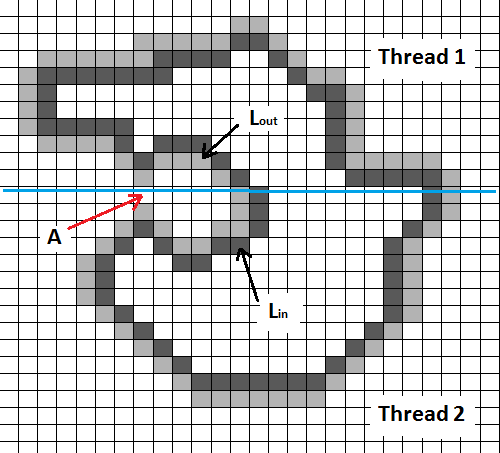
\includegraphics[width=0.6\textwidth]{./imagenes/mismoVecino}
 	\caption{Ejemplo de condici\'{o}n de carrera al querer a\~{n}adir un punto vecino en com\'{u}n a puntos tratados por distintos \textit{threads}}	
 	\label{mismoVecino}
 \end{figure}

\subsection{Primera implementaci\'{o}n}

En esta secci\'{o}n se explican las caracter\'{i}sticas de la primera implementaci\'{o}n paralela realizada siguiendo el an\'{a}lisis del anterior apartado. As\'{i} pues, cada ciclo quedar\'{a} estructurado como se ve en la figura \ref{1-Imple}. Las nuevas caracter\'{i}sticas son de color rojo y se han marcado con un asterisco(*). 

 \begin{figure}[H]
 	\captionsetup{justification=centering}
 	\centering
 	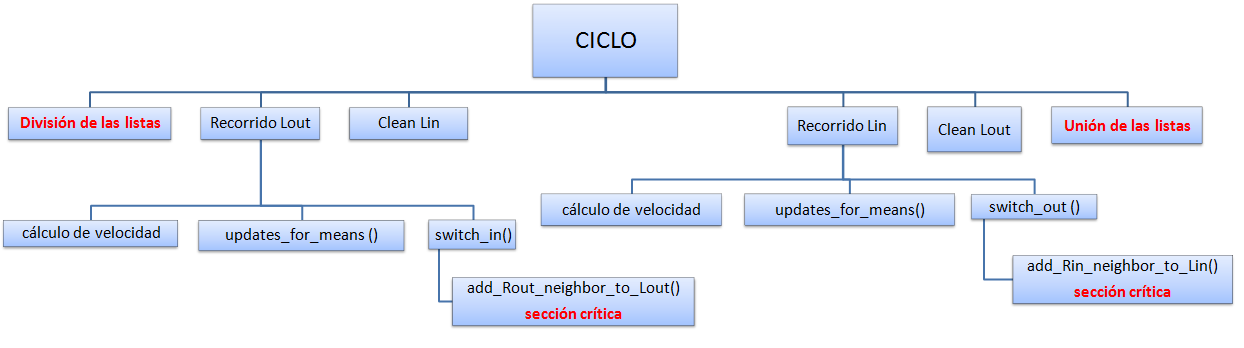
\includegraphics[width=1.2\textwidth]{./imagenes/1-Imple}
 	\caption{Esquema de la primera implementaci\'{o}n}	
 	\label{1-Imple}
 \end{figure}

En esta primera implementaci\'{o}n se invirti\'{o} mucho tiempo ya que los cambios realizados fueron muchos. Se ir\'{a} paso a paso comentando las caracter\'{i}sticas de cada cambio, as\'{i} como la raz\'{o}n por la que se llevo a cabo dicho cambio.

\subsubsection{Lista enlazada}

Muchos han sido los cambios realizados en comparaci\'{o}n con la implementaci\'{o}n de lista enlazada creada en el trabajo Ofeli. Todos los cambios aqu\'{i} realizados han tenido como objetivo minimizar el coste operacional de las operaciones necesarias para realizar la paralelizaci\'{o}n. 

\begin{enumerate}
	\item Se ha insertado en cada nodo un puntero hacia el elemento anterior, es decir, se ha creado una lista doblemente ligada. 
	\item La modificaci\'{o}n anterior ha dado pie a crear un apuntador al final de la lista, un \textit{tail}.
	\item Se ha convertido el tiempo de la ejecuci\'{o}n de la funci\'{o}n size() en orden constante en lugar de la implementaci\'{o}n computacionalmente lineal (al n\'{u}mero de elementos de la lista) que estaba.
	\item Otras modificaciones que no influyen en la implementaci\'{o}n paralela.
\end{enumerate}

\subsubsection{Divisi\'{o}n de la lista}

Las listas $L_{out}$ y $L_{in}$ se dividen en un n\'{u}mero de trozos o sublistas igual al n\'{u}mero de \textit{threads} de manera que cada uno tenga la parte de la lista original con la que trabajar\'{a}. 

Al inicio del programa, despu\'{e}s de inicializar las dos listas con el contorno definido manualmente, se crean tantos punteros o apuntadores como \textit{threads} vayan a trabajar en la ejecuci\'{o}n. Cada puntero se coloca apuntando al primer elemento que tratar\'{a} cada \textit{thread}, es decir, suponiendo que tenemos 80 elementos a repartir entre cuatro \textit{threads}, el primer puntero apuntar\'{a} al primer elemento, ya que ser\'{a} el primer elemento a tratar por el primer \textit{thread}, el segundo puntero apuntar\'{a} al vig\'{e}simo primer elemento y as\'{i} sucesivamente. V\'{e}ase la figura \ref{divisionLista1} para ver un ejemplo de ello. Esta primera recolocaci\'{o}n de los \textit{heads} de cada \textit{thread} se realiza en tiempo lineal al n\'{u}mero de elementos en las listas, sin embargo, esta operaci\'{o}n s\'{o}lo se realiza en la preparaci\'{o}n de la evoluci\'{o}n y por lo tanto, una sola vez. 

 \begin{figure}[H]
 	\captionsetup{justification=centering}
 	\centering
 	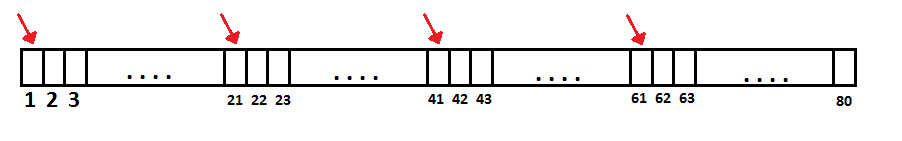
\includegraphics[width=1\textwidth]{./imagenes/divisionLista1}
 	\caption{Esquema de la colocaci\'{o}n de los \textit{heads} de trozo de lista a crear}	
 	\label{divisionLista1}
 \end{figure}
 
 
Por lo tanto, se accede en un orden constante a cada elemento \textit{head} creado, se establecen los \textit{tails} de las sublistas accediendo al anterior elemento de estos \textit{heads}, se establecen los tama\~{n}os de cada sublista (posible conociendo la posici\'{o}n de cada \textit{tail} y llevando una cuenta) y se <<rompen>> los enlaces con sus anteriores elementos de manera que se separen por completo las sublistas. Todo ello es posible gracias a las modificaciones realizadas en la implementaci\'{o}n de la lista ligada. V\'{e}ase la figura \ref{divisionLista2} para ver un ejemplo de todo ello. 

 \begin{figure}[H]
 	\captionsetup{justification=centering}
 	\centering
 	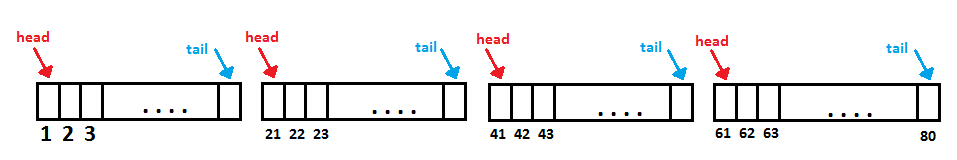
\includegraphics[width=1\textwidth]{./imagenes/divisionLista2}
 	\caption{Ejemplo de creaci\'{o}n de cada sublista usando los \textit{heads} establecidos}	
 	\label{divisionLista2}
 \end{figure} 
 
 
\subsubsection{Uni\'{o}n de las sublistas} 

Siguiendo el procedimiento inverso a la divisi\'{o}n de las listas se realiza la uni\'{o}n. En este caso, sabiendo los \textit{heads} y los \textit{tails} de cada sublista, se vuelve a crear la uni\'{o}n entre ellas, m\'{a}s concretamente, entre el \textit{tail} y el \textit{head} de la siguiente lista. El tama\~{n}o de la lista completa ser\'{a} la suma de los tama\~{n}os de todas las sublistas. V\'{e}ase la figura \ref{unionLista1} como explicaci\'{o}n de ello.

 \begin{figure}[H]
 	\captionsetup{justification=centering}
 	\centering
 	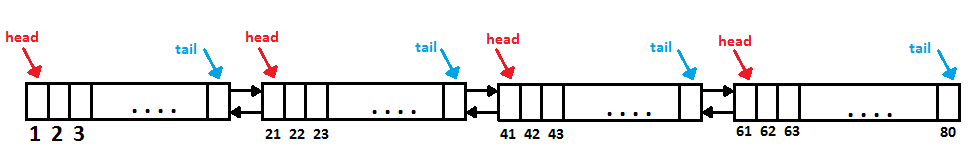
\includegraphics[width=1\textwidth]{./imagenes/unionLista1}
 	\caption{Ejemplo de uni\'{o}n de cada sublista usando los \textit{heads} y \textit{tails} de cada una}	
 	\label{unionLista1}
 \end{figure} 
 
Al realizar esta uni\'{o}n, tambi\'{e}n se aprovecha a reinicializar los \textit{heads} que se utilizar\'{a}n en la siguiente divisi\'{o}n de la lista. Los \textit{heads} se inicializar\'{a}n previamente como los \textit{heads} de cada sublista. N\'{o}tese que estos \textit{heads} se habr\'{a}n posicionado muy cerca de la posici\'{o}n \'{o}ptima, ya que habitualmente todas las zonas del contorno tienden a expandirse por igual. No obstante, se realiza un centrado de cada \textit{head}, es decir, se mueve el puntero hasta la posici\'{o}n exacta en la que debe estar, si es que no lo est\'{a}, realizando la divisi\'{o}n del n\'{u}mero de puntos entre el n\'{u}mero de \textit{thread} de la ejecuci\'{o}n. Los \textit{tails} no har\'{a}n falta establecerlos ya que se posicionan en la divisi\'{o}n de las listas. V\'{e}ase la figura \ref{unionLista2} como explicaci\'{o}n de ello. El n\'{u}mero de operaciones a realizar comparadas con el n\'{u}mero de puntos en la lista es peque\~{n}o.

 \begin{figure}[H]
 	\captionsetup{justification=centering}
 	\centering
 	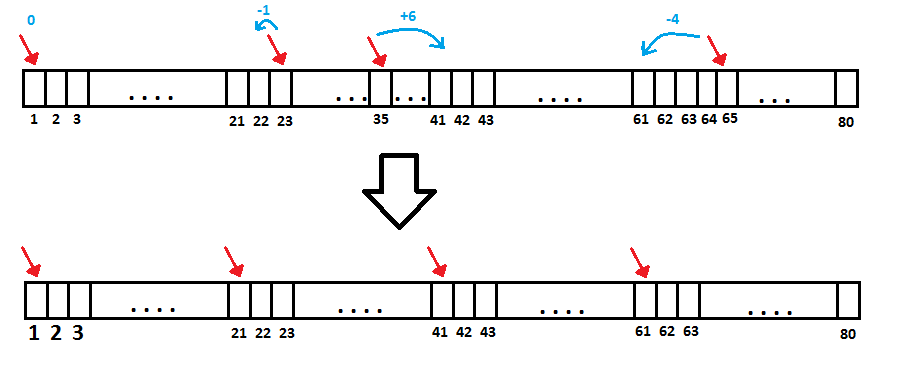
\includegraphics[width=1\textwidth]{./imagenes/unionLista2}
 	\caption{Ejemplo de uni\'{o}n de cada sublista usando los \textit{heads} y \textit{tails} de cada una}	
 	\label{unionLista2}
 \end{figure}
 
 
 
 \subsubsection{Secciones cr\'{i}ticas} 
 
 Las secciones cr\'{i}ticas a realizar para resolver la condici\'{o}n de carrera se han establecido en las funciones de a\~{n}adir un vecino del punto que se cambia de una lista a otra. Se ha seguido un esquema \textit{Test and Test-and-set} para minimizar la contenci\'{o}n de la secci\'{o}n cr\'{i}tica ya que se realiza antes la condici\'{o}n que se debe de hacer en la secci\'{o}n cr\'{i}tica antes de entrar a \'{e}sta.
 
 A continuaci\'{o}n se presenta el c\'{o}digo de la secci\'{o}n cr\'{i}tica.


\subsubsection{C\'{o}digo}

\begin{lstlisting}
void ActiveContour::add_Rout_neighbor_to_Lout(int neighbor_offset,int tid)
{
	//Test, test and set
	if( phi[neighbor_offset] == 3 ) // exterior value
	{
		#pragma omp critical
		{
			if( phi[neighbor_offset] == 3 ) // exterior value
			{
				phi[neighbor_offset] = 1; // outside boundary value
	
				Splited_Lout[tid]->push_front(neighbor_offset);	
			}
		}
	}	
return;}

void ActiveContour::add_Rin_neighbor_to_Lin(int neighbor_offset,int tid)
{
	//Test, test and set
	if( phi[neighbor_offset] == -3 ) // interior value
	{
		#pragma omp critical
		{
			if( phi[neighbor_offset] == -3 ) // interior value
			{
				phi[neighbor_offset] = -1; // inside boundary value
			
				Splited_Lin[tid]->push_front(neighbor_offset);
			}
		}
	}	
return;}	
\end{lstlisting}

 
\subsection{Rendimiento}
 
Realizada la primera implementaci\'{o}n, llega la hora de comprobar su rendimiento y ver la mejora obtenida respecto a la versi\'{o}n serie. En estas primeras pruebas se ha utilizado \'{u}nicamente una imagen de tama\~{n}o 3000x2800 y que es exactamente la que se muestra en la figura \ref{ejemplo4}.

Las pruebas realizadas han sido en un ordenador de la Universidad del Pa\'{i}s Vasco. Este ordenador tiene una arquitectura SMP, con una memoria principal de 64GB y dispone de cuatro procesadores \textit{AMD Opteron(tm) Processor 6168} los cuales tienen doce \textit{cores} que trabajan a 1900 MHz. Por lo tanto, se disponen de 48 \textit{cores} para poder realizar las pruebas. Tambi\'{e}n se ha considerado a\~{n}adir que se ha tenido que separar la parte gr\'{a}fica del trabajo original de Ofeli y extraer el algoritmo de evoluci\'{o}n para poder realizar las pruebas. 

La compilaci\'{o}n se ha realizado con el compilador gcc (versi\'{o}n 4.6.3) con la siguiente l\'{i}nea de comandos:

\

\quad \quad \textbf{g++ main.cpp activecontour.cpp ac\_withoutedges.cpp -o prueba}

\quad \quad	\textbf{-O3 -fopenmp -Dcimg\_use\_png -lpng -lz -Dcimg\_display=0}

\

Mientras no se diga lo contrario, todas las ejecuciones se realizar\'{a}n en la misma m\'{a}quina y los tiempos de todas las tablas que aparezcan ser\'{a}n la media de cinco ejecuciones. A esta primera implementaci\'{o}n se le nombrar\'{a} como <<secci\'{o}n critica normal>>.


\begin{table}[h]
	\small
	\centering
	\captionsetup{justification=centering}
	\begin{tabular}{cccccccc}
		\hline
		\multicolumn{1}{|c|}{{\bf N\'{u}mero de threads}} & \multicolumn{1}{c|}{{\bf Serie}} & \multicolumn{1}{c|}{{\bf 2}} & \multicolumn{1}{c|}{{\bf 4}} & \multicolumn{1}{c|}{{\bf 8}} & \multicolumn{1}{c|}{{\bf 16}} & \multicolumn{1}{c|}{{\bf 32}} & \multicolumn{1}{c|}{{\bf 48}} \\ \hline
		\multicolumn{1}{|c|}{{\bf Tiempo (s)}}           & \multicolumn{1}{c|}{16,52}      & \multicolumn{1}{c|}{11,63}  & \multicolumn{1}{c|}{7,80}   & \multicolumn{1}{c|}{9,38}   & \multicolumn{1}{c|}{14,37}   & \multicolumn{1}{c|}{27,66}   & \multicolumn{1}{c|}{31,37}   \\ \hline
		\multicolumn{1}{l}{}                         & \multicolumn{1}{l}{}             & \multicolumn{1}{l}{}         & \multicolumn{1}{l}{}         & \multicolumn{1}{l}{}         & \multicolumn{1}{l}{}          & \multicolumn{1}{l}{}          & \multicolumn{1}{l}{}          \\ \hline
		\multicolumn{1}{|c|}{{\bf Speed-up}}         & \multicolumn{1}{c|}{1,00}        & \multicolumn{1}{c|}{1,42}    & \multicolumn{1}{c|}{2,12}    & \multicolumn{1}{c|}{1,76}    & \multicolumn{1}{c|}{1,15}     & \multicolumn{1}{c|}{0,60}     & \multicolumn{1}{c|}{0,53}     \\ \hline
		{\bf }                                       &                                  &                              &                              &                              &                               &                               &                               \\ \hline
		\multicolumn{1}{|c|}{{\bf Eficiencia}}       & \multicolumn{1}{c|}{100,00\%}    & \multicolumn{1}{c|}{71,03\%} & \multicolumn{1}{c|}{52,98\%} & \multicolumn{1}{c|}{22,02\%} & \multicolumn{1}{c|}{7,19\%}   & \multicolumn{1}{c|}{1,87\%}   & \multicolumn{1}{c|}{1,10\%}   \\ \hline
	\end{tabular}
	\caption{Rendimiento de las ejecuciones de la primera implementaci\'{o}n paralela}
\end{table}	


\begin{figure}[H]
 	\captionsetup{justification=centering}
 	\centering
 	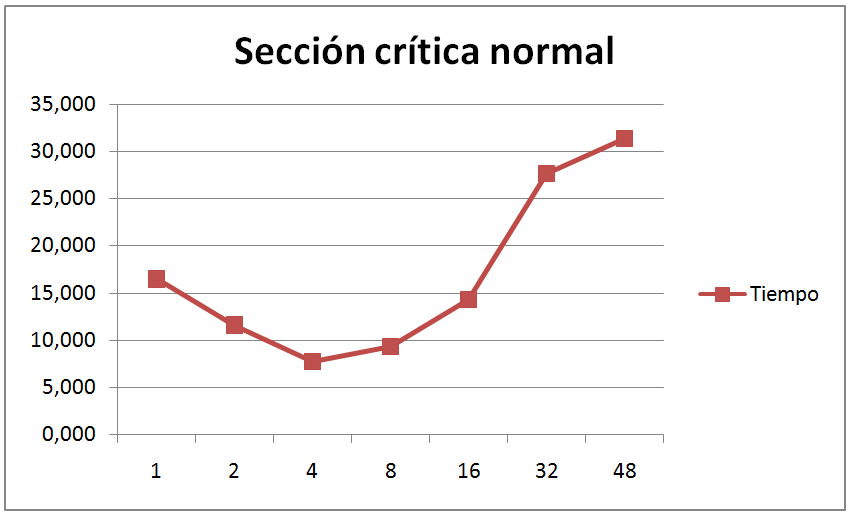
\includegraphics[width=.7\textwidth]{./imagenes/grafico1Imple}
 	\caption{Gr\'{a}fica de los tiempos de ejecuci\'{o}n de la primera implementaci\'{o}n paralela}	
 	\label{grafico1Imple}
\end{figure}

Como se puede observar en la figura \ref{grafico1Imple}, esta primera implementaci\'{o}n s\'{o}lo escala bien hasta los cuatro \textit{cores}. 

\subsubsection{Conclusi\'{o}n}

Se analizan los tiempos de ejecuci\'{o}n y se comprueba que, efectivamente, el cuello de botella est\'{a} en el acceso a la secci\'{o}n cr\'{i}tica. V\'{e}ase el desglose del tiempo de ejecuci\'{o}n (2 \textit{cores}) de un ciclo en la tabla \ref{tablaConclusiones1}. Aqu\'{i} se puede observar que la mayor\'{i}a del tiempo se pierde en realizar los bucles 1 y 2, es decir, donde est\'{a}n las funciones con la secciones cr\'{i}ticas. Esto sucede ya que \'{e}sta se hace pr\'{a}cticamente siempre, debido a que el contorno suele tender a expandirse, y puede que se repita varias veces por cada punto, al realizarse por cada nuevo vecino. Por otro lado, la ejecuci\'{o}n es \'{u}nicamente con dos \textit{cores}, por lo que la contenci\'{o}n de la secci\'{o}n cr\'{i}tica ser\'{a} mayor con m\'{a}s \textit{cores}, raz\'{o}n por la que esta primera implementaci\'{o}n no escala bien.

\begin{table}[H]
	\centering
	\small
	\captionsetup{justification=centering}
	\begin{tabular}{c|c|c|c|c|c|c|c}
		\cline{2-8}
		\multicolumn{1}{l|}{}                          & {\bf \begin{tabular}[c]{@{}c@{}}Divisi\'{o}n\\   listas\end{tabular}} & {\bf  \begin{tabular}[c]{@{}c@{}}1º\\   bucle\end{tabular}} & {\bf \begin{tabular}[c]{@{}c@{}}Clean\\   Lin\end{tabular}} & {\bf  \begin{tabular}[c]{@{}c@{}}2º\\   bucle\end{tabular}} & {\bf \begin{tabular}[c]{@{}c@{}}Clean\\   Lout\end{tabular}} & {\bf \begin{tabular}[c]{@{}c@{}}Uni\'{o}n\\   listas\end{tabular}} & \multicolumn{1}{c|}{{\bf \begin{tabular}[c]{@{}c@{}}POR\\   CICLO\end{tabular}}} \\ \hline
		\multicolumn{1}{|c|}{{\bf Serie}}              & 0,0                  & 0,0127       & 0,008         & 0,0145       & 0,0071         & 0,0                                                               & \multicolumn{1}{c|}{0,043}         \\ \hline
		\multicolumn{1}{|c|}{{\bf \begin{tabular}[c]{@{}c@{}}\'{O}ptimo 2\\   threads\end{tabular}}}   & 0,0                  & 0,0063       & 0,0040        & 0,0072       & 0,0035         & 0,0                                                              & \multicolumn{1}{c|}{0,0215}        \\ \hline
		\multicolumn{1}{|c|}{{\bf \begin{tabular}[c]{@{}c@{}}Paralelo 2\\   threads\end{tabular}}} & 0,0                  & 0,0093       & 0,0041        & 0,0109       & 0,0038         & 0,0                                                               & \multicolumn{1}{c|}{0,0281}        \\ \hline
		\multicolumn{1}{|c|}{{\bf Sobrecoste}}           & 0,0\%                    & 46,0\%         & 2,1\%           & 51,3\%         & 8,6\%            & 0,0\%                                                                 & \multicolumn{1}{l}{}                 \\ \cline{1-7}
	\end{tabular}
	\caption{Desglose de tiempos (s) de un ciclo del algoritmo con una ejecuci\'{o}n paralela con dos \textit{cores} de la primera implementaci\'{o}n}		
	\label{tablaConclusiones1}
\end{table}


\section{Primer paso de mejora: segunda implementaci\'{o}n}

Concluido ya que el problema est\'{a} en la secci\'{o}n cr\'{i}tica se intenta reducir las operaciones dentro de \'{e}sta reduciendo as\'{i} el tiempo que cada \textit{thread} est\'{a} dentro de ella. La <<secci\'{o}n cr\'{i}tica mejorada>> tendr\'{a} \'{u}nicamente dos asignaciones, reduciendo considerablemente el tiempo dentro de ella. Se utilizar\'{a} un \textit{flag} para saber qu\'{e} \textit{thread} ha sido el que ha entrado a la secci\'{o}n cr\'{i}tica para posteriormente hacer la operaci\'{o}n correspondiente. En este caso obviaremos la segunda funci\'{o}n ya que tiene las mismas caracter\'{i}sticas que la primera.

\subsubsection{C\'{o}digo}

\begin{lstlisting}

 void ActiveContour::add_Rout_neighbor_to_Lout(int neighbor_offset,int tid)
 {
 	bool flag = false;
 	
 	if( phi[neighbor_offset] == 3 ) // exterior value
 	{
 		#pragma omp critical
 		{
 			if( phi[neighbor_offset] == 3 ) // exterior value
 			{
 				phi[neighbor_offset] = 1; // outside boundary value
 				flag = true;
 			}
 		}
 		if(flag)  Splited_Lout[tid]->push_front(neighbor_offset);
 	} 	
 	return; 
 }
 	
\end{lstlisting}

\subsection{Rendimiento}

\begin{table}[H]
	\small
	\centering
	\captionsetup{justification=centering}
	\begin{tabular}{cccccccc}
		\hline
		\multicolumn{1}{|c|}{{\bf N\'{u}m. \textit{threads}}} & \multicolumn{1}{c|}{{\bf Serie}} & \multicolumn{1}{c|}{{\bf 2}} & \multicolumn{1}{c|}{{\bf 4}} & \multicolumn{1}{c|}{{\bf 8}} & \multicolumn{1}{c|}{{\bf 16}} & \multicolumn{1}{c|}{{\bf 32}} & \multicolumn{1}{c|}{{\bf 48}} \\ \hline
		\multicolumn{1}{|c|}{{\bf Tiempo (s)}}           & \multicolumn{1}{c|}{16,52}      & \multicolumn{1}{c|}{10,74}  & \multicolumn{1}{c|}{6,58}   & \multicolumn{1}{c|}{5,42}   & \multicolumn{1}{c|}{3,68}    & \multicolumn{1}{c|}{6,02}    & \multicolumn{1}{c|}{6,79}    \\ \hline
		\multicolumn{1}{l}{}                         & \multicolumn{1}{l}{}             & \multicolumn{1}{l}{}         & \multicolumn{1}{l}{}         & \multicolumn{1}{l}{}         & \multicolumn{1}{l}{}          & \multicolumn{1}{l}{}          & \multicolumn{1}{l}{}          \\ \hline
		\multicolumn{1}{|c|}{{\bf Speed-up}}         & \multicolumn{1}{c|}{1,00}        & \multicolumn{1}{c|}{1,54}    & \multicolumn{1}{c|}{2,51}    & \multicolumn{1}{c|}{3,05}    & \multicolumn{1}{c|}{4,49}     & \multicolumn{1}{c|}{2,74}     & \multicolumn{1}{c|}{2,43}     \\ \hline
		{\bf }                                       &                                  &                              &                              &                              &                               &                               &                               \\ \hline
		\multicolumn{1}{|c|}{{\bf Eficiencia}}       & \multicolumn{1}{c|}{100,0\%}    & \multicolumn{1}{c|}{76,9\%} & \multicolumn{1}{c|}{62,8\%} & \multicolumn{1}{c|}{38,1\%} & \multicolumn{1}{c|}{28,1\%}  & \multicolumn{1}{c|}{8,6\%}   & \multicolumn{1}{c|}{5,1\%}   \\ \hline
	\end{tabular}
	\caption{Rendimiento obtenido de las ejecuciones de la segunda implementaci\'{o}n paralela}
\end{table}




\begin{figure}[H]
	\captionsetup{justification=centering}
	\centering
	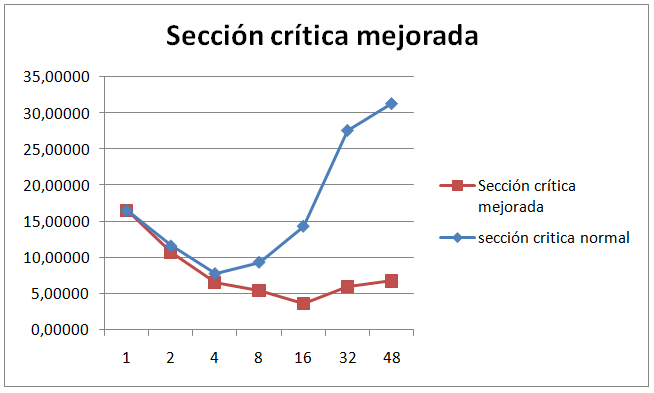
\includegraphics[width=.8\textwidth]{./imagenes/grafico2Imple}
	\caption{Gr\'{a}fica de los tiempos de ejecuci\'{o}n de la primera y segunda implementaci\'{o}n}	
	\label{grafico2Imple}
\end{figure}

Como se puede ver en el gr\'{a}fico \ref{grafico2Imple} la mejora es bastante notable. Esto se debe a que se ha reducido notablemente la contenci\'{o}n entre los \textit{threads} al no tener pr\'{a}cticamente operaciones a realizar dentro de la secci\'{o}n cr\'{i}tica. El tiempo de ejecuci\'{o}n del sistema se reduce hasta los 16 cores.

\


\subsubsection{Conclusi\'{o}n}

A pesar de haber mejorado mucho los tiempos el resultado no sigue siendo \'{o}ptimo del todo ya que la implementaci\'{o}n escala poco a poco hasta los 16 \textit{threads} y luego el tiempo va aumentado. Hay que intentar reducir a\'{u}n m\'{a}s la contenci\'{o}n de alguna manera. Analizando un poco m\'{a}s a detalle, la secci\'{o}n cr\'{i}tica se realiza para cualquier vecino que se quiera a\~{n}adir despu\'{e}s de haber expandido o contra\'{i}do un punto. Es decir, que no importa la localizaci\'{o}n de los puntos que se est\'{e}n tratando, habr\'{a} colisi\'{o}n en la secci\'{o}n cr\'{i}tica. En realidad, la secci\'{o}n cr\'{i}tica se puso para evitar que se pudieran a\~{n}adir varios puntos vecinos a la vez. ¿Hay alguna manera de realizar secciones cr\'{i}ticas dependientes del punto? Ser\'{i}a la pregunta clave a responder para poder resolver el problema. 

\section{Segundo paso de mejora: tercera implementaci\'{o}n}

Buscando alguna manera de realizar secciones cr\'{i}ticas dependiente del punto se deciden usar sem\'{a}foros o \textit{locks} en ingl\'{e}s. Se podr\'{i}a tener una matriz de \textit{locks} de la misma dimensi\'{o}n que la imagen y cada vez que se vaya a trabajar con un punto cerrar el \textit{lock} que le pertenece. El problema de esta idea de tener un \textit{lock} para cada p\'{i}xel, en una imagen de 3000x2800, ser\'{i}a la cantidad de memoria y la complejidad de gesti\'{o}n de \'{e}stos, ya que el n\'{u}mero de \textit{locks} necesarios ser\'{i}a muy elevado. Como alternativa y buscando una soluci\'{o}n de compromiso se ha implementado un esquema de \textit{locks} por zonas. En vez de tener un \textit{lock} para cada punto se podr\'{i}a tener un n\'{u}mero de \textit{locks} no muy grande para bloquear cierta zona de la imagen. 

\begin{figure}[H]
	\captionsetup{justification=centering}
	\centering
	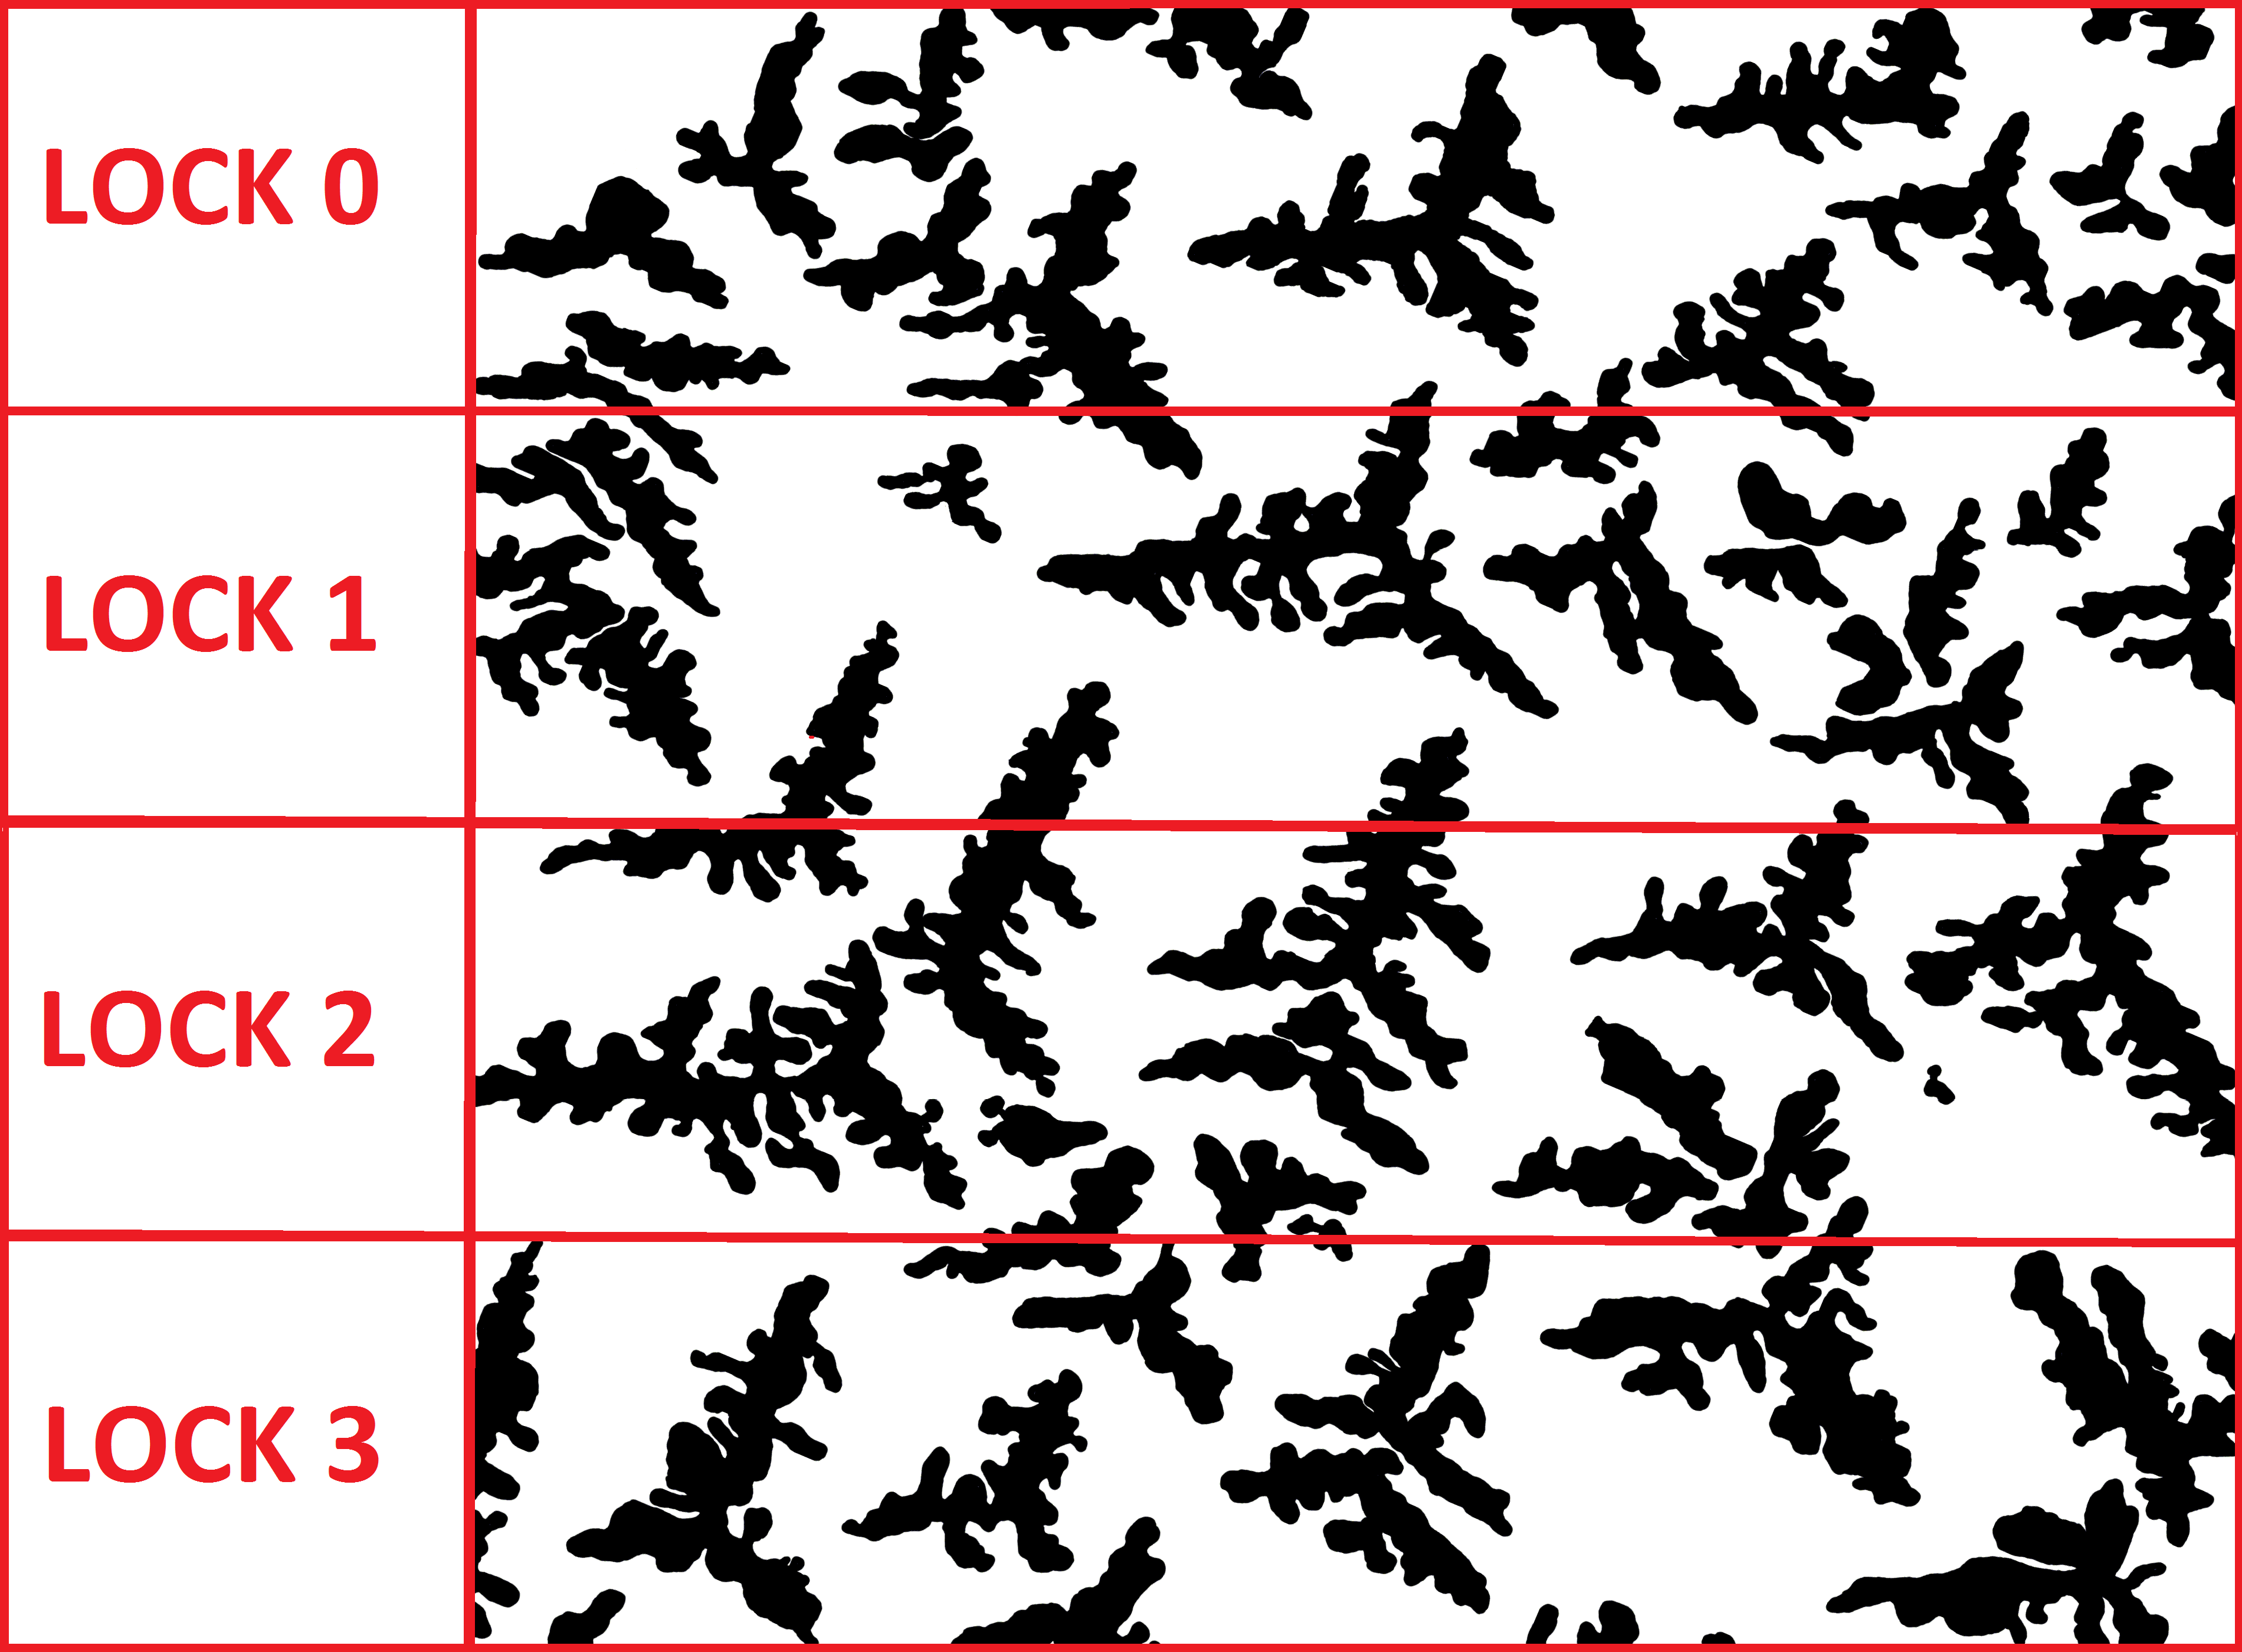
\includegraphics[width=.7\textwidth]{./imagenes/mallaLocks}
	\caption{Ejemplo de una malla de cuatro locks de establecidos en forma rectangular}	
	\label{mallaLocks}
\end{figure}

En la imagen \ref{mallaLocks} se puede observar un ejemplo de una malla de \textit{locks} en la n\'{u}mero de \textit{locks} establecido es 4 y tiene una forma rectangular. El n\'{u}mero de \'{o}ptimo de locks a establecer ser\'{a} lo que se trabaje en esta tercera implementaci\'{o}n. Adem\'{a}s, el lector podr\'{i}a pensar que se pueden realizar distintas figuras geom\'{e}tricas en la creaci\'{o}n de la estructura de \textit{locks}, aunque esta opci\'{o}n no se realizar\'{a} en este proyecto ya que la estrategia de distribuci\'{o}n de los puntos en las sublistas se realiza recorriendo la matriz por filas, lo que significa que los rect\'{a}ngulos dar\'{a}n una mejor respuesta temporal ya que habr\'{a} poca colisi\'{o}n entre los \textit{threads}.

\subsubsection{C\'{o}digo}

\begin{lstlisting}
void ActiveContour::add_Rout_neighbor_to_Lout(int neighbor_offset,int tid)
{
	bool flag = false;	
	
	if( phi[neighbor_offset] == 3 ) // exterior value
	{
		int lockNumber = ( (neighbor_offset/img_width) *numLocks)/img_height;
					
		omp_set_lock(&(locks[lockNumber]));	
					
		if( phi[neighbor_offset] == 3 ) // exterior value
		{
			phi[neighbor_offset] = 1; // outside boundary value
			flag = true;
		}	
		
		omp_unset_lock(&(locks[lockNumber]));	
		
		if(flag)  Splited_Lout[tid]->push_front(neighbor_offset);
	}
	return;	
}
\end{lstlisting}


\subsection{Rendimiento}


\begin{table}[H]
	\centering
	\captionsetup{justification=centering}
	\begin{tabular}{lc|c|c|c|c|c|c|lcccl}
		\cline{3-8}
		& \multicolumn{1}{l|}{} & \multicolumn{6}{c|}{{\bf Locks}}                              &                       & \multicolumn{1}{l}{}          & \multicolumn{1}{l}{}  & \multicolumn{1}{l}{}            &  \\ \cline{3-8} \cline{10-10} \cline{12-12}
		&                       & {\bf 4} & {\bf 8} & {\bf 16} & {\bf 24} & {\bf 32} & {\bf 50} & \multicolumn{1}{l|}{} & \multicolumn{1}{c|}{{\bf su}} & \multicolumn{1}{c|}{} & \multicolumn{1}{c|}{{\bf Efi.}} &  \\ \cline{1-8} \cline{10-10} \cline{12-12}
		\multicolumn{1}{|l|}{\multirow{13}{*}{{\bf \rotatebox[origin=c]{90}{THREADS}}}} & {\bf 1}               & 16,69   & 16,64   & 16,63    & 16,61    & 16,79    & 16,73    & \multicolumn{1}{l|}{} & \multicolumn{1}{c|}{-}        & \multicolumn{1}{c|}{} & \multicolumn{1}{c|}{-}          &  \\ \cline{2-8} \cline{10-10} \cline{12-12}
		\multicolumn{1}{|l|}{}                                & {\bf 2}               & 10,49   & 10,64   & 10,35    & 10,52    & 10,35    & 10,33    & \multicolumn{1}{l|}{} & \multicolumn{1}{c|}{1,59}     & \multicolumn{1}{c|}{} & \multicolumn{1}{c|}{79,6\%}     &  \\ \cline{2-8} \cline{10-10} \cline{12-12}
		\multicolumn{1}{|l|}{}                                & {\bf 4}               & 6,79    & 7,03    & 6,86     & 6,85     & 6,73     & 6,60     & \multicolumn{1}{l|}{} & \multicolumn{1}{c|}{2,46}     & \multicolumn{1}{c|}{} & \multicolumn{1}{c|}{61,5\%}     &  \\ \cline{2-8} \cline{10-10} \cline{12-12}
		\multicolumn{1}{|l|}{}                                & {\bf 8}               & 4,22    & 5,73    & 5,72     & 5,42     & 5,44     & 5,40     & \multicolumn{1}{l|}{} & \multicolumn{1}{c|}{3,96}     & \multicolumn{1}{c|}{} & \multicolumn{1}{c|}{49,5\%}     &  \\ \cline{2-8} \cline{10-10} \cline{12-12}
		\multicolumn{1}{|l|}{}                                & {\bf 12}               & 4,10    & 4,63    & 4,31     & 4,53     & 5,11     & 5,12     & \multicolumn{1}{l|}{} & \multicolumn{1}{c|}{4,07}     & \multicolumn{1}{c|}{} & \multicolumn{1}{c|}{33,9\%}     &  \\ \cline{2-8} \cline{10-10} \cline{12-12}
		\multicolumn{1}{|l|}{}                                & {\bf 16}              & 3,99    & 3,93    & 4,89     & 3,26     & 4,87     & 4,84     & \multicolumn{1}{l|}{} & \multicolumn{1}{c|}{4,18}     & \multicolumn{1}{c|}{} & \multicolumn{1}{c|}{26,1\%}     &  \\ \cline{2-8} \cline{10-10} \cline{12-12}
		\multicolumn{1}{|l|}{}                                & {\bf 20}              & 3,29    & 3,87    & 3,88     & 3,19     & 3,89     & 3,89     & \multicolumn{1}{l|}{} & \multicolumn{1}{c|}{5,08}     & \multicolumn{1}{c|}{} & \multicolumn{1}{c|}{25,4\%}     &  \\ \cline{2-8} \cline{10-10} \cline{12-12}
		\multicolumn{1}{|l|}{}                                & {\bf 24}              & 2,95    & 3,28    & 3,29     & 3,32     & 3,30     & 3,29     & \multicolumn{1}{l|}{} & \multicolumn{1}{c|}{5,65}     & \multicolumn{1}{c|}{} & \multicolumn{1}{c|}{23,5\%}     &  \\ \cline{2-8} \cline{10-10} \cline{12-12}
		\multicolumn{1}{|l|}{}                                & {\bf 28}              & 3,03    & 2,96    & 2,93     & 2,92     & 2,96     & 2,93     & \multicolumn{1}{l|}{} & \multicolumn{1}{c|}{5,52}     & \multicolumn{1}{c|}{} & \multicolumn{1}{c|}{19,7\%}     &  \\ \cline{2-8} \cline{10-10} \cline{12-12}
		\multicolumn{1}{|l|}{}                                & {\bf 32}              & 2,85    & 2,72    & 2,80     & 2,70     & 3,00     & 2,80     & \multicolumn{1}{l|}{} & \multicolumn{1}{c|}{5,86}     & \multicolumn{1}{c|}{} & \multicolumn{1}{c|}{18,3\%}     &  \\ \cline{2-8} \cline{10-10} \cline{12-12}
		\multicolumn{1}{|l|}{}                                & {\bf 36}              & 3,74    & 3,81    & 3,29     & 3,48     & 2,85     & 3,28     & \multicolumn{1}{l|}{} & \multicolumn{1}{c|}{4,46}     & \multicolumn{1}{c|}{} & \multicolumn{1}{c|}{12,4\%}     &  \\ \cline{2-8} \cline{10-10} \cline{12-12}
		\multicolumn{1}{|l|}{}                                & {\bf 40}              & 4,12    & 4,06    & 3,79     & 3,98     & 3,85     & 3,81     & \multicolumn{1}{l|}{} & \multicolumn{1}{c|}{4,05}     & \multicolumn{1}{c|}{} & \multicolumn{1}{c|}{10,1\%}     &  \\ \cline{2-8} \cline{10-10} \cline{12-12}
		\multicolumn{1}{|l|}{}                                & {\bf 44}              & 4,00    & 4,06    & 4,05     & 3,83     & 3,75     & 3,74     & \multicolumn{1}{l|}{} & \multicolumn{1}{c|}{4,18}     & \multicolumn{1}{c|}{} & \multicolumn{1}{c|}{9,5\%}      &  \\ \cline{2-8} \cline{10-10} \cline{12-12}
		\multicolumn{1}{|l|}{}                                & {\bf 48}              & 3,91    & 3,91    & 3,77     & 3,68     & 3,82     & 3,66     & \multicolumn{1}{l|}{} & \multicolumn{1}{c|}{4,27}     & \multicolumn{1}{c|}{} & \multicolumn{1}{c|}{8,9\%}      &  \\ \cline{1-8} \cline{10-10} \cline{12-12}
	\end{tabular}
	\caption{Tiempos de ejecuci\'{o}n (s),  eficiencia y \textit{speed-ups} (su) obtenidos con distintas combinaciones de \textit{threads} y \textit{locks} en la tercera implementaci\'{o}n paralela}
\end{table}

\begin{figure}[H]
	\captionsetup{justification=centering}
	\centering
	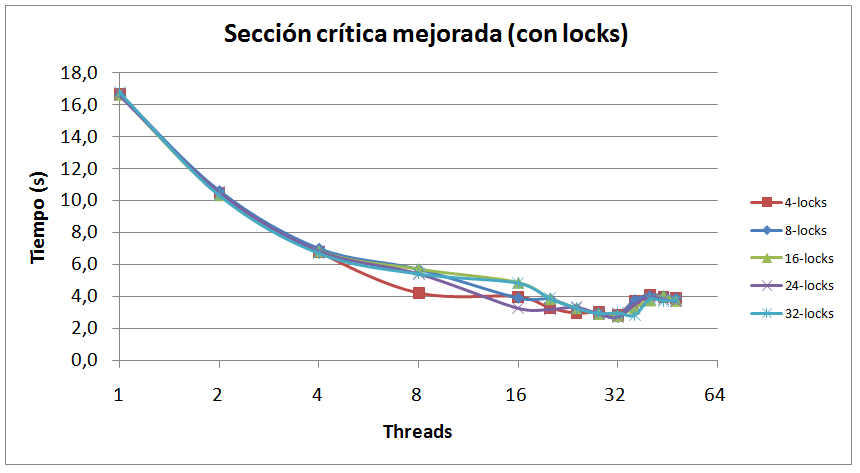
\includegraphics[width=0.8\textwidth]{./imagenes/grafico3Imple}
	\caption{Gr\'{a}fico de los resultados obtenidos en este tercera implementaci\'{o}n}
	\label{Implementacion3}
\end{figure}

Como se puede observar en la figura \ref{Implementacion3} se ha mejorado a\'{u}n m\'{a}s la respuesta temporal, escala bien hasta los 32 \textit{threads} en vez de hasta los 16 que se consegu\'{i}an con la anterior implementaci\'{o}n (v\'{e}ase la figura \ref{grafico2Imple}). Las ejecuciones m\'{a}s r\'{a}pidas se logran con la combinaci\'{o}n de 32 \textit{threads} y con 24 \textit{locks}, teniendo un resultado de 2,7 segundos. 

Por otro lado, tambi\'{e}n se han realizado pruebas con la primera implementaci\'{o}n, es decir, con la <<secci\'{o}n cr\'{i}tica normal>> para analizar el efecto de la reducci\'{o}n de la contenci\'{o}n mediante la soluci\'{o}n de \textit{locks} distribuidos en dicha implementaci\'{o}n. Esto se refiere a que la secci\'{o}n la crear\'{a}n los \textit{locks} pero lo que hay dentro ser\'{a} lo que hab\'{i}a en la implementaci\'{o}n de la <<secci\'{o}n cr\'{i}tica normal>>. Los resultados son los que se muestran en el gr\'{a}fico \ref{grafico3-2Imple}. Como se puede observar el tiempo obtenido es pr\'{a}cticamente el conseguido con la \'{u}ltima implementaci\'{o}n realizada. Esto quiere decir que el problema de todo ello era la contenci\'{o}n que hab\'{i}a con todos los \textit{threads} y no importa tanto el tiempo que se pasa dentro de la secci\'{o}n cr\'{i}tica. Sin embargo, tambi\'{e}n ah\'{i} que decir que con la implementaci\'{o}n de la <<secci\'{o}n cr\'{i}tica normal>> son necesarios m\'{a}s \textit{locks} para evitar esa contenci\'{o}n entre los \textit{threads} ya que la secci\'{o}n cr\'{i}tica es m\'{a}s larga.

\begin{figure}[H]
	\captionsetup{justification=centering}
	\centering
	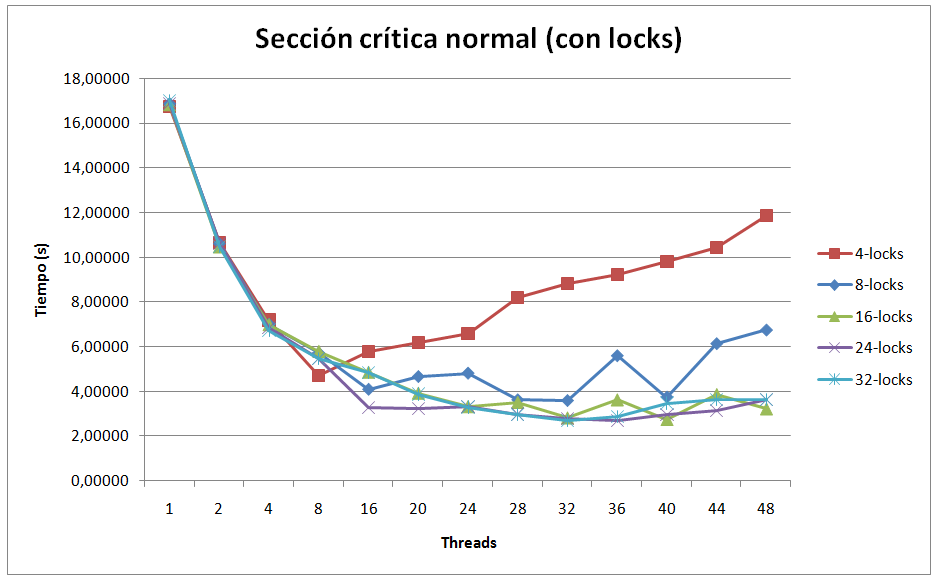
\includegraphics[width=.9\textwidth]{./imagenes/grafico3-2Imple}
	\caption{Gr\'{a}fica de los tiempos de ejecuci\'{o}n con los \textit{locks} y la estructura de la <<secci\'{o}n cr\'{i}tica normal>>}	
	\label{grafico3-2Imple}
\end{figure}


\subsubsection{Conclusi\'{o}n}

Ya que los resultados obtenidos con la \'{u}ltima implementaci\'{o}n y la primera son parecidos no se podr\'{a} reducir mucho m\'{a}s el tiempo en cuanto a la contenci\'{o}n, ya que parece que a partir de cierto n\'{u}mero de \textit{locks} \'{e}sta desaparece. As\'{i} pues, la reducci\'{o}n tendr\'{i}a que hacerse por otra v\'{i}a, o bien intentar reducir el tiempo que se realiza en paralelo o entrar en m\'{a}s detalle como la compartici\'{o}n falsa en la memoria cach\'{e} que pudiera haber con ciertas variables de la implementaci\'{o}n. El propio tiempo de gesti\'{o}n de los \textit{locks}, la compartici\'{o}n falsa en cach\'{e} que pudiera haber con ciertas variables, la gesti\'{o}n de la secci\'{o}n paralela y la divisi\'{o}n y uni\'{o}n de las listas parece que a\~{n}aden en total un \textit{overhead} que se ha decidido dejar fuera del \'{a}mbito de este proyecto. 

En el ap\'{e}ndice \ref{apendice1} se puede encontrar el c\'{o}digo de los ciclos principales de la evoluci\'{o}n del algoritmo \textit{level set}, piezas principales de la implementaci\'{o}n paralela realizada. 